\section{Regresión lineal simple y múltiple}
\begin{itemize}[label=\color{red}\textbullet, leftmargin=*]
	\item \color{lightblue}Introducción
\end{itemize}
\lb{Objetivo:} predecir una variable numérica a partir de $k$ variables numéricas (variables predictoras) minimizando el error en la predicción.

Para ello necesitamos disponer de una muestra en la que se conozcan dichas variables (aprendizaje supervisado), esta muestra se usará para elegir el mejor modelo y para validar su fiabilidad.
\begin{itemize}[label=\color{red}\textbullet, leftmargin=*]
	\item \color{lightblue}Planteamiento
\end{itemize}
Se trata de predecir el valor (numérico) de una \va (v.a.) $Y$ a partir de unas variables predictoras $X_1,\dots,X_k$.

Para ello usaremos una función predictora lineal \[ h_\theta(x_1,\dots,x_k)\coloneq\theta_0+\theta_1x_1+\cdots+\theta_kx_k, \] donde $\theta=(\theta_0,\dots,\theta_k)'\in\R^{k+1}$ serán los parámetros del modelo que se deben elegir de forma que la estimación de $Y$ sea óptima (el error sea mínimo).
\begin{itemize}[label=\color{lightblue}$\to$]
\item Una sola variable predictora $\longrightarrow$ \lb{Regresión lineal simple}.
\item Más de una variable predictora $\longrightarrow$ \lb{Regresión lineal múltiple}.
\end{itemize}

\subsection{Estimación de los parámetros}
\subsubsection{Muestra}
Para ello necesitamos disponer de una muestra (\lb{training sample}) de esas $k+1$ variables sobre $n$ individuos.

Una realización de la muestra se denotará como \[ \left(x_1^{(i)},\dots,x_k^{(i)},y^{(i)}\right),\quad i=1,\dots,n, \] que equivale a la notación introducida en el tema anterior \[ (x_{i,1},\dots,x_{i,k},y_i),\quad i=1,\dots,n. \]
Los datos se representan en forma de tabla:
\[ \begin{array}{cccccc}
i & x_1 & x_2 & \cdots & x_k & y \\ \hline
\mathbf{o}_1 & x_1^{(1)} & x_2^{(1)} & \cdots & x_k^{(1)} & y_1 \\
\cdots & \cdots & \cdots & \cdots & \cdots & \cdots \\
\mathbf{o}_i & x_1^{(i)} & x_2^{(i)} & \cdots & x_k^{(i)} & y_i \\
\cdots & \cdots & \cdots & \cdots & \cdots & \cdots \\
\mathbf{o}_n & x_1^{(n)} & x_2^{(n)} & \cdots & x_k^{(n)} & y_n \\ \hline
\end{array}\qquad\begin{array}{cccccc}
i & x_1 & x_2 & \cdots & x_k & y \\ \hline
\mathbf{o}_1 & x_{1,1} & x_{1,2} & \cdots & x_{1,k} & y_1 \\
\cdots & \cdots & \cdots & \cdots & \cdots & \cdots \\
\mathbf{o}_i & x_{i,1} & x_{i,2} & \cdots & x_{i,k} & y_i \\
\cdots & \cdots & \cdots & \cdots & \cdots & \cdots \\
\mathbf{o}_n & x_{n,1} & x_{n,2} & \cdots & x_{n,k} & y_n \\ \hline
\end{array} \]

\subsection{Conjunto de datos \textbf{\texttt{USArrests}}}

\subsubsection*{Cargamos los datos}
Podemos visualizar los datos con \code{view(d)} y las primeras filas con \code{head(d)}.

\begin{lstlisting}
d <- USArrests
head(d, n = 6)
\end{lstlisting}

\begin{verbatim}
##            Murder Assault UrbanPop Rape
## Alabama      13.2     236       58 21.2
## Alaska       10.0     263       48 44.5
## Arizona       8.1     294       80 31.0
## Arkansas      8.8     190       50 19.5
## California    9.0     276       91 40.6
## Colorado      7.9     204       78 38.7
\end{verbatim}
\subsubsection*{¿Qué información está recogida en el conjunto de datos?}
Con la instrucción \code{help(USArrests)} conocemos qué información está contenida en el conjunto:
\begin{itemize}
\item \code{Murder:} Ratios de arrestos por asesinatos por cada $100\,000$ residentes en cada uno de los 50 estados de la unión.
\item \code{Assault:} Ratios de arrestos por agresión por cada $100\,000$ residentes en cada uno de los 50 estados de la unión.
\item \code{UrbanPop:} Porcentaje de población que vive en áreas urbanas.
\item \code{Rape:} Ratios de arrestos por violación por cada $100\,000$ residentes en cada uno de los 50 estados de la unión.
\end{itemize}
\subsubsection{Objetivo}

Predecir el ratio de arrestos por asesinatos ($Y=$\code{Murder}) en función de la variable $X=$\code{UrbanPop}.

\begin{wrapfigure}[3]{r}{0.4\textwidth}

\begin{tikzpicture}
	\node[red, draw=red, fill=red!10, line width=1.5, text width=\linewidth] {Podemos observar que no parece existir ninguna relación entre las variables \texttt{Murder} y \texttt{UrbanPop} por lo que la predicción no será muy buena.};
\end{tikzpicture}
\end{wrapfigure}

Para visualizar la relación entre estas variables podemos representarlas situando $X$ en el eje horizontal e $Y$ en el vertical.

\begin{lstlisting}
x <- d$UrbanPop #Elegimos x
y <- d$Murder #Elegimos y
plot(x, y, xlab = 'UrbanPop', ylab = 'Murder')
\end{lstlisting}

\begin{center}
\includegraphics[scale=0.7]{"Temas/Imágenes/Tema 2/000005"}
\end{center}

\newpage

\begin{wrapfigure}[4]{r}{0.4\textwidth}

\begin{tikzpicture}
	\node[red, draw=red, fill=red!10, line width=1.5, text width=\linewidth] {Ahora sí se aprecia una relación lineal (creciente entre ambas variables.)};
\end{tikzpicture}
\end{wrapfigure}

Si usamos como predictor la variable \code{Assault} y representamos gráficamente:

\begin{lstlisting}
x <- d$Assault #Elegimos x
y <- d$Murder #Elegimos y
plot(x, y, xlab = 'Assault', ylab = 'Murder')
\end{lstlisting}

\begin{center}
\includegraphics[scale=0.7]{"Temas/Imágenes/Tema 2/000010"}
\end{center}

\subsubsection{Matriz de gráficos}
Podemos representar conjuntamente todas las variables con gráficos bidimensionales para cada pareja de variables.

\begin{lstlisting}
plot(d)
\end{lstlisting}

\begin{center}
\includegraphics[scale=0.7]{"Temas/Imágenes/Tema 2/000002"}
\end{center}
\subsubsection{Resumen numérico de las variables}
Podemos obtener los estadísticos descriptivos de estas variables con \code{summary(d)} que incluyen los extremos (mínimo y máximo), los cuartiles, la mediana y la media.
\begin{lstlisting}
summary(d)
\end{lstlisting}
\begin{verbatim}
##      Murder          Assault         UrbanPop          Rape
##  Min.   : 0.800   Min.   : 45.0   Min.   :32.00   Min.   : 7.30
##  1st Qu.: 4.075   1st Qu.:109.0   1st Qu.:54.50   1st Qu.:15.07
##  Median : 7.250   Median :159.0   Median :66.00   Median :20.10
##  Mean   : 7.788   Mean   :170.8   Mean   :65.54   Mean   :21.23
##  3rd Qu.:11.250   3rd Qu.:249.0   3rd Qu.:77.75   3rd Qu.:26.18
##  Max.   :17.400   Max.   :337.0   Max.   :91.00   Max.   :46.00
\end{verbatim}
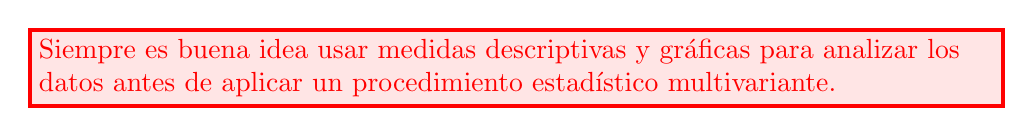
\begin{tikzpicture}
	\node[red, draw=red, fill=red!10, line width=1.5, text width=\linewidth] {Siempre es buena idea usar medidas descriptivas y gráficas para analizar los datos antes de aplicar un procedimiento estadístico multivariante.};
\end{tikzpicture}
\subsubsection{Estimación de las varianzas y covarianzas}
Para calcular una estimación de las varianzas y covarianzas utilizaremos la función \code{var} (\code{R} obtiene las cuasivarianzas).

\begin{lstlisting}
#calculo directo de la varianza y cuasivarianza para Murder
mu <- mean(d$Murder)
n <- length(d)
hat_sigma = sum((d$Murder-mu)^ 2)/n #varianza muestral
S = sum((d$Murder-mu)^ 2)/(n-1) #cuasivarianza muestral
#calculo de la matriz de covarianzas
var(d)
\end{lstlisting}

\begin{verbatim}
##              Murder   Assault   UrbanPop      Rape
## Murder    18.970465  291.0624   4.386204  22.99141
## Assault  291.062367 6945.1657 312.275102 519.26906
## UrbanPop   4.386204  312.2751 209.518776  55.76808
## Rape      22.991412  519.2691  55.768082  87.72916
\end{verbatim}

\subsubsection{Modelo completo}

Podemos incluir todas las variables en el modelo considerado \[ h_\theta=\theta_0+\theta_1\text{Assault}+\theta_2\text{UrbanPop}+\theta_3\text{Rape} \]donde $\theta=(\theta_0,\theta_1,\theta_2,\theta_3)'\in\R^4$ son los parámetros del modelo que debemos ajustar para obtener las mejores aproximaciones posibles.

Los casos en los que solo usamos una variable están incluidos en este modelo haciendo que los parámetros de las otras variables sean cero.

También podemos intentar mejorar estas aproximaciones considerando otras funciones $h$ (no lineales).

\subsection{Regresión lineal simple}
\subsubsection{Modelo teórico}
Partiremos de un \vea $(X,Y)$.

\lb{Objetivo:} Construir una nueva variable $h(X)$ que se \lb{parezca} (aproxime) a $Y$.

Los errores (residuos) serán otra variable aleatoria \[ R=Y-h(X) \](notemos que pueden ser positivos o negativos).

Existen diversas reglas para determinar una función objetivo que mida cómo son esos errores y trate de minimizarlos.

La más usada es el denominado \lb{error cuadrático medio} (EMC) definido como: \[ EMC=E\left[(h(X)-Y)^2\right] \] (MSE, \lb{Mean Square Error})

\subsubsection{Función óptima}

Supongamos que $(X,Y)$ tiene una distribución absolutamente continua con función de densidad conjunta $f$ y marginales $f_X$ y $f_Y$.

Entonces se puede demostrar que la función $h$ que \lb{minimiza} el $EMC$ es \[ h_{\mathrm{opt}}(x)=E(Y|X=x)=\infi yf_{Y|X}(y|x)\dy, \]donde\[ f_{Y|X}(y|x)=f(x,y)|f_X(x), \] para tales $f_X(x)>0$, es la \lb{función de densidad condicionada} de $(Y|X=x)$.

Esta función se denomina \lb{curva de regresión} y es el mejor predictor de $Y$ dado $X$ según el $ECM$.
\subsection{Caso de normalidad}
El vector $(X,Y)$ tiene una distribución normal $\mathcal{N}_2(\mu,V)$:

$\mu=(\mu_1,\mu_2)'$ es el vector de medias ($A'$ representa la traspuesta de la matriz $A$), donde \[ \begin{array}{l}
\mu_1=\mu_X=E[X]\\
\mu_2=\mu_Y=[Y]
\end{array} \]
$V=\begin{pmatrix}
\sigma_{1,1} & \sigma_{1,2}\\
\sigma_{2,1} & \sigma_{2,2}\\
\end{pmatrix}$ es la matriz de varianzas-covarianzas, donde \[ \begin{array}{l}
\sigma_{1,1}=\sigma_X^2=\var(X)=E[(X-\mu_X)^2],\\
\sigma_{2,2}=\sigma_Y^2=\var(Y)=E[(Y-\mu_Y)^2],\\
\sigma_{1,2}=\sigma_{2,1}=\sigma_{X,Y}=\cov(X,Y)=E[(X-\mu_X)(Y-\mu_Y)].
\end{array} \]

Entonces la \lb{distribución condicionada} $(Y|X=x)$ se comporta también como una \lb{distribución normal}, \[ (Y|X=x)\longrightarrow \mathcal{N}_1(\overline{\mu},\overline{\sigma}^2), \] con \[ \begin{array}{c}
\begin{aligned}
h_{\mathrm{opt}}(x)=\overline{\mu}&=E(Y|X=x)=\mu_2+\dfrac{\sigma_{1,2}}{\sigma_{1,1}}(x-\mu_1)\\
&=\mu_Y+\dfrac{\cov(X,Y)}{\sigma_X^2}(x-\mu_X)
\end{aligned}\\
\overline{\sigma}^2=\var(Y|X=x)=\sigma_{2,2}-\dfrac{\sigma_{1,2}^2}{\sigma_{1,1}}=\sigma_Y^2-\dfrac{\cov(X,Y)^2}{\sigma_X^2}.
\end{array} \]

\begin{itemize}[label=\color{red}\textbullet, leftmargin=*]
	\item \color{lightblue}Observaciones
\end{itemize}
Bajo la hipótesis de normalidad, la \lb{curva de regresión} $h_{\mathrm{opt}}$ es siempre una \lb{recta} y la varianza $\overline{\sigma}^2$ no depende de $x$.

Los residuos condicionados $R_x=R|X=x$ también serán normales $R_x\longrightarrow \mathcal{N}(0,\overline{\sigma}^2)$ e idénticamente distribuidos.

La \lb{curva (recta) de regresión} para predecir $Y$ en función de $X$ se puede escribir como \[ \dfrac{y-\mu_Y}{\sigma_Y}=\rho_{X,Y}\dfrac{x-\mu_X}{\sigma_X}, \]donde $\rho_{X,Y}=\dfrac{\cov(X,Y)}{\sigma_X\sigma_Y}$ es el \lb{coeficiente de correlación lineal de Pearson}.

La recta siempre pasa por el punto $(\mu_X,\mu_Y)$.
\subsubsection{Coeficiente de correlación de Pearson}
\begin{itemize}[label=\color{red}\textbullet, leftmargin=*]
	\item \color{lightblue}Propiedades
\end{itemize}
El \lb{signo de la pendiente de la recta} de regresión siempre coincide con el signo de $\rho_{X,Y}$.

Se verifica que: \[ \overline{\sigma}^2=\sigma_Y^2-\dfrac{\cov(X,Y)^2}{\sigma_X^2\sigma_Y^2}\sigma_Y^2=(1-\rho_{X,Y}^2)\sigma_Y^2\ge0, \]por lo que $-1\le\rho_{X,Y}\le1$.

Cuando $\rho_{X,Y}=\pm1$ tendremos ajustes perfectos con residuos nulos.

La recta (curva) para predecir $X$ a partir de $Y$ se calcula de forma similar y no coincide con la curva para predecir $Y$ a partir de $X$ que acabamos de calcular salvo cuando $\rho_{X,Y}=\pm1$.
\subsection{Caso de no normalidad}
\begin{itemize}[label=\color{red}\textbullet, leftmargin=*]
	\item \color{lightblue}Observaciones
\end{itemize}
Para otras distribuciones bivariantes la curva de regresión no tiene por qué ser una recta.\\
Cuando $X$ e $Y$ sean independientes, $Y$ e $(Y|X=x)$ tienen la misma distribución y la curva óptima \[ h_{\mathrm{opt}}(x)=E(Y|X=x)=E(Y) \] es constante (por lo que también es una recta).
\begin{itemize}[label=\color{lightblue}$\to$]
\item En este caso el valor de $X$ no influye en la predicción sobre $Y$.
\item $\rho_{X,Y}=0$ (recta horizontal).
\end{itemize}
\subsection{Restricción sobre la función $h$}
En \textbf{Regresión Lineal Simple} supondremos que la función $h$ es una recta
\begin{itemize}
\item Limitamos nuestra función $h$ a una recta, es decir, \[ h_\theta(x)\coloneq\theta_0+\theta_1x \]
\item Usamos como criterio minimizar el ECM.
\item El objetivo será \[ \min_{\theta_0,\theta_1}J(\theta_0,\theta_1), \] donde \[ J(\theta_0,\theta_1)\coloneq E[(h_\theta(X)-Y)^2]=E[(\theta_0+\theta_1X+Y)^2] \]se conoce como \lb{función costo} y $J(\theta_0,\theta_1)\ge0$.
\begin{itemize}[label=\color{lightblue}$\to$]
\item Por lo tanto, se trata de minimizar una función costo
\end{itemize}
\end{itemize}
\subsection{Minimizar la función costo}
\subsubsection{Ecuaciones normales de la recta}
La función $J(\theta)$ es convexa por lo que tendrá un único mínimo que se puede obtener resolviendo el sistema \[ \begin{array}{l}
\dfrac{\partial J(\theta_0,\theta_1)}{\partial\theta_0}=2E[\theta_0+\theta_1X-Y]=0\\
\dfrac{\partial J(\theta_0,\theta_1)}{\partial\theta_1}=2E[(\theta_0+\theta_1X-Y)X]=0\\
\end{array} \]
Estas ecuaciones se conocen como \lb{ecuaciones normales}.

De la primera ecuación obtenemos \[ \theta_0=E(Y)-\theta_1E(X) \](con lo que la recta pasará por el punto formado con las medias).

De la segunda \[ \theta_0E(X)+\theta_1E(X^2)=E(XY) \]
Y sustituyendo la primera en la segunda, se obtiene \[ E(X)E(Y)-\theta_1E^2(X)+\theta_1E(X^2)=E(XY), \]es decir, \[ \theta_1\var(X)=\cov(X,Y), \]puesto que $\var(X)=E(X^2)-E^2(X)$ y $\cov(X,Y)=E(XY)-E(X)E(Y)$.

Con lo cual,
\begin{itemize}[label=\color{lightblue}$\to$]
\item $\hat{\theta}_1=\dfrac{\cov(X,Y)}{\var(X)}=\dfrac{\sigma_{X,Y}}{\sigma_X^2}$
\item $\hat{\theta}_0=E(Y)-\hat{\theta}_1E(X)=E(Y)-E(X)\dfrac{\cov(X,Y)}{\var(X)}=\mu_Y-\mu_X\dfrac{\sigma_{X,Y}}{\sigma_X^2}$
\end{itemize}
\subsection{Expresión de la recta}
\subsubsection{Recta de regresión para predecir $Y$ en función de $X$}
En el punto $(\hat{\theta}_0,\hat{\theta}_1)$ se alcanza el mínimo de la función $J$, \[ \min_{\theta_0,\theta_1}J(\theta_0,\theta_1)=J(\hat{\theta}_0,\hat{\theta}_1) \]
Expresión de la recta: \[ h_{\hat{\theta}}(x)=\mu_Y-\mu_X\dfrac{\sigma_{X,Y}}{\sigma_X^2}+\dfrac{\sigma_{X,Y}}{\sigma_X^2}x=\mu_Y+\dfrac{\sigma_{X,Y}}{\sigma_X^2}(x-\mu_X). \] (Note que la fórmula es la misma que la de la curva de regresión de la normal).

Otra expresión: \[ \dfrac{y-\mu_Y}{\sigma_Y}=\rho_{X,Y}\dfrac{x-\mu_X}{\sigma_X} \]donde $\rho_{X,Y}=\dfrac{\sigma_{X,Y}}{\sigma_X\sigma_Y}$ es el \lb{coeficiente de correlación lineal de Pearson}.

La \va \[ \hat{Y}=h_{\hat{\theta}}(X)=\hat{\theta}_0+\hat{\theta}_1X \]se usará para estimar $Y$.

Los residuos se definen como $R=Y-\hat{Y}$.

Se verifica:
\begin{itemize}[label=\color{lightblue}$\to$]
\item $E(\hat{Y})=E(Y)$
\item $E(R)=0$
\end{itemize}
\subsection{Descomposición de la varianza}
\subsubsection{Relaciones entre las varianzas}
Expresando $Y=\hat{Y}+R$, se tiene que: \[ \sigma_y=\var(Y)=\var(\hat{Y})+\var(R) \]
Puesto que \[ \begin{array}{c}
\var(\hat{Y})=\hat{\theta}_1^2\sigma_X^2=\dfrac{\sigma_{X,Y}P2}{\sigma_X^2}=\rho_{X,Y}^2\sigma_Y^2\\
\var(R)=\var(Y-\hat{\theta}_1X)=(1-\rho_{X,Y}^2)\sigma_Y^2.
\end{array} \]
Es decir, la información (varianza) contenida en $Y$ se descompone como \[ \sigma_Y^2=\rho_{X,Y}^2\sigma_Y^2+(1-\rho_{X,Y}^2)\sigma_Y^2. \]
\subsection{Coeficiente de determinación}
\begin{itemize}[label=\color{red}\textbullet, leftmargin=*]
	\item \color{lightblue}Definición
\end{itemize}
El \lb{coeficiente de determinación} $d_{X,Y}=\rho_{X,Y}^2$ es el porcentaje (en tanto por 1) de la información de $Y$ explicada por la recta de regresión (por relaciones lineales de $X$). Denotado habitualmente en los paquetes estadísticos por $R^2$.

Análogamente, $1-d_{X,Y}=1-\rho_{X,Y}^2$ indicaría la parte de $Y$ no explicada por esa recta y que se queda en el residuo.

Además, se tiene que \[ E(\hat{Y}R)=0, \] es decir, la variable que se obtiene con la recta de regresión y los residuos son incorrelados.

Bajo normalidad, ambas variables serán normales (por ser combinaciones lineales de $X$ e $Y$) y, por lo tanto, serán independientes.
\subsection{Inferencia y predicción}
\begin{itemize}[label=\color{red}\textbullet, leftmargin=*]
	\item \color{lightblue}Una muestra
\end{itemize}
En la práctica tanto la distribución conjunta (densidad) de $(X,Y)$ como todas esas medidas serán desconocidas por lo que tendrán que ser estimadas a partir de una muestra de esas variables (\lb{training sample}).

Si la muestra es grande, podemos extraer algunos datos (no usados en el cálculo de la recta) para comprobar cómo de fiables serán nuestras estimaciones.

La muestra se denotará como \[ \left(x^{(i)},y^{(i)}\right),\quad i=1,\dots,n, \]donde $n$ será el tamaño muestral.

Los datos de cada variable se representarán como columnas y todos lo datos como una matriz $D$.
\subsection{Función costo empírica}
\subsubsection{Objetivo}
Queremos aproximar los valores de $Y$ mediante una recta (función lineal) de $X$, es decir, \[ h_\theta\coloneq\theta_0+\theta_1x, \]donde $\mathbf{\theta}=(\theta_0,\theta_1)$ son parámetros desconocidos.

Para calcular estos parámetros minimizaremos una función coste empírica $J$ que nos mida el error cometido.

La más utilizada es el \lb{error cuadrático medio} (o una función proporcional a él), por ejemplo podemos considerar \[ J(\theta_0,\theta_1)\coloneq\dfrac{1}{2n}\sum_{i=1}^{n}\left(h_\theta\left(x^{(i)} \right) - y^{(i)}\right)^2=\dfrac{1}{2n}\sum_{i=1}^{n}\left(\theta_0+\theta_1x^{(i)}-y^{(i)}\right)^2 \]
El objetivo es minimizar esta función en $\R^2$.


\subsubsection{Diferenciar $J$}

Para obtener la solución exacta debemos diferencias $J$ con respecto a los parámetros obteniendo \[ \begin{array}{l}
	\dfrac{\partial}{\partial \theta_0}J(\theta_0,\theta_1)=\dfrac{1}{n}\sum_{i=1}^{n}\left(h\theta\left(x^{(i)}\right)-y^{(i)}\right)\\
	\dfrac{\partial}{\partial\theta_1}J(\theta_0,\theta_1)=\dfrac{1}{n}\sum_{i=1}^{n}\left(h_\theta\left(x^{(i)}\right)-y^{(i)}\right)x^{(i)}
\end{array} \]
Igualando a cero obtenemos las \lb{ecuaciones normales empíricas}:

$\begin{array}{l}
	\dfrac{\partial}{\partial \theta_0}J(\theta_0,\theta_1)=\dfrac{1}{n}\sum_{i=1}^{n}\left(h\theta\left(x^{(i)}\right)-y^{(i)}\right)=\dfrac{1}{n}\sum_{i=1}^{n}\left(\theta_0+\theta x^{(i)}-y^{(i)}\right)\cdot1=0\\
	\dfrac{\partial}{\partial\theta_1}J(\theta_0,\theta_1)=\dfrac{1}{n}\sum_{i=1}^{n}\left(h_\theta\left(x^{(i)}\right)-y^{(i)}\right)x^{(i)}=\dfrac{1}{n}\sum_{i=1}^{n}\left(\theta_0+\theta_1x^{(i)}-y^{(i)}\right)x^{(i)}=0
\end{array}$
\subsubsection{Solución exacta}
De la primera ecuación, \[ \theta_0+\theta_1\overline{x}-\overline{y}=0 \]donde $\overline{x}=\dfrac{1}{n}\sum_{i=1}^{n}x^{(i)}$ e $\overline{y}=\dfrac{1}{n}\sum_{i=1}^{n}y^{(i)}$ son las medias muestrales de $x$ e $y$, respectivamente.

La solución óptima pasa por el punto medio $(\overline{x},\overline{y})$ (individuo promedio).

De la segunda, \[ \theta_0\overline{x}+\theta_1a(x,x)-a(x,y)=0,\] donde $a(x,x)=\dfrac{1}{n}\sum_{i=1}^{n}\left(x^{(i)}\right)^2$ y $a(x,y)=\dfrac{1}{n}\sum_{i=1}^{n}x^{(i)}y^{(i)}$.

Resolviendo este sistema de ecuaciones obtenemos \[ \theta_1\left(a(x,x)-(\overline{x})^2\right)=a(x,y)-\overline{xy} \]
Obtenemos: \[ \hat{\theta}_1=\dfrac{s_{x,y}}{s_x^2},\quad \hat{\theta}_0=\overline{y}-\hat{\theta}_1\overline{x}, \] donde $s_{x,y}=a(x,y)-\overline{xy}=\dfrac{1}{n}\sum_{i=1}^{n}x^{(i)}y^{(i)}-\overline{xy}=\dfrac{1}{n}\sum_{i=1}^{n}\left(x^{(i)}-\overline{x}\right)\left(y^{(i)}.\overline{y}\right)$ es la covarianza muestral y $s_x^2=a(x,x)-(\overline{x})^2=\dfrac{1}{n}\sum_{i=1}^{n}\left(x^{(i)}\right)^2-(\overline{x})^2=\dfrac{1}{n}\sum_{i=1}^{n}\left(x^{(i)}-\overline{x}\right)^2$ es la varianza muestral de $x$.

Supondremos que $s_x^2$ no es cero, es decir, que $x$ presenta más de un valor. Si no, el sistema tendría infinitas soluciones.

Puede comprobarse que $J$ es convexa y por lo tanto la solución que hemos obtenido de las ecuaciones normales empíricas es un mínimo local.
\begin{itemize}[label=\color{lightblue}$\to$]
	\item Además, como es único y $J$ es continua, se trata del único mínimo global.
\end{itemize}

\subsubsection*{¿Es un mínimo local?}
Las segundas derivadas parciales son \[ \begin{array}{l}
	D_{1,1}=\dfrac{\partial^2}{\partial\theta_0^2}J(\theta_0,\theta_1)=\dfrac{1}{n}\sum_{i=1}^{n}1=1\\
	D_{1,2}=\dfrac{\partial^2}{\partial\theta_0\theta_1}J(\theta_0,\theta_1)=\dfrac{1}{n}\sum_{i=1}^{n}x^{(i)}=\overline{x}\\
	D_{2,2}=\dfrac{\partial}{\partial\theta_1^2}J(\theta_0,\theta_1)=\dfrac{1}{n}\sum_{i=1}^{n}\left(x^{(i)}\right)^2=a(x,x)
\end{array} \]
Se verifica que $D_{1,1}=1>0$ y si $D=(D_{i,j})$ es la matriz con esas derivadas, tenemos \[ |D|=\begin{vmatrix}
	1 & \overline{x}\\
	\overline{x} & a(x,x)
\end{vmatrix}=a(x,x)-(\overline{x})^2=s_x^2>0 \]por lo que el punto sería un mínimo local de $J$.


\begin{tikzpicture}
	\node[red, draw=red, fill=red!10, line width=1.5, text width=\linewidth] {
	Como es el único mínimo local en $\R$ y $J$ es continua, será el único mínimo global.

	La solución óptima empírica coincide con la que obtendríamos sustituyendo en la solución teórica las medias, varianzas y covarianzas por sus estimaciones.
	};
\end{tikzpicture}
\subsection{Regresión lineal múltiple}
\subsubsection{Modelo teórico}
En el caso general queremos \lb{predecir} $Y$ (o $X_{k+1}$) a partir de $k$ variables $X_1,\dots,X_k$ (sobre el mismo espacio de probabilidad).

En el modelo lineal queremos construir una función \[ h_\theta(x_1,\dots,x_k)\coloneq\theta_0+\theta_1x_1+\cdots+\theta_kx_K, \]de forma que $h_\theta(X_1,\dots,X_k)$ esté lo más cerca posible de $Y$.

Para \lb{medir el error} usaremos de nuevo el \lb{error cuadrático medio} \[ EMC(\theta)=E\left[(h_\theta(X_1,\dots,X_k)-Y)^2\right]. \]
Si consideramos una nueva variable constante (degenerada) $X_0=1$, podemos escribir ese error como \[ ECM(\theta)=E\left[(\mathbf{\theta'X}-Y)^2\right], \] donde $\mathbf{X}=(X_0,X_1,\dots,X_k)'$ y $\mathbf{\theta'}=(\theta_0,\theta_1,\dots,\theta_k)\in\R^{k+1}$.
\subsubsection{Obtención del mínimo}
Como en el caso $k=1$ se puede comprobar que esta función es convexa por lo que tendrá un único minimo $\hat{\theta}'\in\R^{k+1}$.

Para detectarlo hacemos las derivadas parciales iguales a cero \[ \dfrac{\partial}{\partial\theta_j}ECM(\mathbf{\theta})=E[2(\theta'\mathbf{X}-Y)X_j]=0 \]
Obteniendo \[ \mathbf{\theta}'E(\mathbf{X}X_j)=E(YX_j), \]para $j=0,\dots,k$, es decir, \[ \mathbf{\theta}'E(\mathbf{XX'})=E(Y\mathbf{X}') \]
O equivalente, \[ E(\mathbf{XX'})\mathbf{\theta}=E(\mathbf{X}Y). \]
Con lo que la solución es \[ \hat{\theta}=(E(\mathbf{XX'}))^{-1}E(\mathbf{X}Y) \]siempre que existe la inversa de la matriz simétrica \[ A=E(\mathbf{XX'})=(E(X_iX_j))_{ij} \]y donde (por convenio)\[ E(\mathbf{X}Y)=(E(X_0Y),\dots,E(X_kY))'. \]
\subsection{Coeficiente de correlación múltiple}
\begin{itemize}[label=\color{red}\textbullet, leftmargin=*]
	\item \color{lightblue}Definición
\end{itemize}
Si $\mathbf{Z}=(X_1,\dots,X_k,Y)'$ es un vector aleatorio se llama \lb{coeficiente de correlación múltiple al cuadrado} de $Y$ respecto de $\mathbf{X}=(X_1,\dots,X_k)'$ a \[ \corr^2(\mathbf{X},Y)=\rho_{k+1,(1,\dots,k)}^2=\dfrac{v_{1,2}'V_\mathbf{X}^{-1}v_{1,2}}{\sigma_Y^2} \]donde $\cov(\mathbf{Z})=\begin{pmatrix}
	V_\mathbf{X} & v_{1,2}\\
	v_{1,2}' & \sigma_Y^2
\end{pmatrix},\:V_\mathbf{X}=\cov(\mathbf{X}),\:\sigma_Y^2=\var(Y),$ y $v_{1,2}'=(\sigma_{1,k+1},\dots,\sigma_{k,k+1})=\cov(X_1,Y),\dots,\cov(X_k,Y)$.

\begin{tikzpicture}
	\node[red, draw=red, fill=red!10, line width=1.5, text width=\linewidth] {\underline{Nota:}
	
	Si $k=1$, es decir, si tenemos el \vea bidimensional $(X,Y)$, entonces el \textbf{coeficiente de correlación múltiple al cuadrado} se corresponde con la \textbf{correlación de Pearson al cuadrado} (de $X$ e $Y$), esto es, \[ \rho_{2,(1)}^2=\dfrac{\sigma_{1,2}\sigma_{1,1}^{-1}\sigma_{1,2}}{\sigma_{2,2}}=\rho_{1,2}^2 \]};
\end{tikzpicture}
\begin{itemize}[label=\color{red}\textbullet, leftmargin=*]
	\item \color{lightblue}Proposición
\end{itemize}
El \lb{coeficiente de correlación múltiple} es el máximo de las correlaciones lineales al cuadrado de $Y$ con combinaciones lineales de $\mathbf{X}=(X_1,\dots,X_k)'$, es decir, \[ \max_{\alpha}\corr^2(Y,\mathbf{\alpha'X})=\rho_{k+1,(1,\dots,k)}^2 \]y ese máximo se obtiene con $\mathbf{\alpha}=\lambda V_\mathbf{X}^{-1}v_{1,2}$, para $\lambda\neq0$.
\begin{itemize}[label=\color{red}\textbullet, leftmargin=*]
	\item \color{lightblue}Demostración
\end{itemize}
De la definición se tiene \[ \begin{aligned}
	\corr^2(Y,\mathbf{\alpha'X})&=\dfrac{(\cov(Y,\mathbf{\alpha'X}))^2}{\sigma_Y^2\var(\mathbf{\alpha'X})}=\dfrac{(\cov(Y,\mathbf{X})\mathbf{\alpha})^2}{\sigma_Y^2\cov(\mathbf{\alpha'X},\mathbf{\alpha'X})}\\
	&=\dfrac{(\mathbf{\alpha'}v_{1,2})^2}{\sigma_Y^2\mathbf{\alpha}V_\mathbf{X}\mathbf{\alpha}}=\dfrac{\left(\mathbf{\alpha'}V_{\mathbf{X}}^{\frac{1}{2}}V_{\mathbf{X}}^{-\frac{1}{2}}v_{1,2}\right)^2}{\sigma_Y^2\mathbf{\alpha'}V_{\mathbf{X}}\mathbf{\alpha}}
\end{aligned} \]
Y usando la desigualdad de Cauchy-Schwarz, para $\mathbf{x'}=\mathbf{\alpha'}V_{\mathbf{X}}^{\frac{1}{2}}$ e $y=V_{\mathbf{X}}^{-\frac{1}{2}}v_{1,2}$, se tiene \[ \corr^2(Y,\mathbf{\alpha'X})\le\dfrac{\mathbf{\alpha'}V_\mathbf{X}\mathbf{\alpha}v_{1,2}'V_\mathbf{X}^{-1}v_{1,2}}{\sigma_Y^2\mathbf{\alpha'}V_{\mathbf{X}}\mathbf{\alpha}}=\dfrac{v_{1,2}'V_{\mathbf{X}}^{-1}v_{1,2}}{\sigma_Y^2}, \]es decir, $\rho_{k+1,(1,\dots,k)}^2$ es un cota superior.

Además, la igualdad en Cauchy-Schwarz se obtiene si y solo si los vectores $\mathbf{x}$ e $\mathbf{y}$ tienen la misma dirección\[ \mathbf{x}=V_{\mathbf{X}}^{-\frac{1}{2}}\alpha=\lambda\mathbf{y}=\lambda V_{\mathbf{X}}^{-\frac{1}{2}}v_{1,2}, \]es decir, si $\mathbf{\alpha}=\lambda V_{\mathbf{X}}^{-1}v_{1,2}$ para $\lambda\neq0$.
\subsubsection{Desigualdad de Cauchy-Schwarz}
Para vectores columna $\mathbf{x,y}\in\R^m$, se verifica \[ (\mathbf{x'y})^2\le(\mathbf{x'x})(\mathbf{y'y}), \]y se obtiene la igualdad si y solo si los vectores $\mathbf{x}$ e $\mathbf{y}$ tienen la misma dirección, esto es, $\mathbf{x}=\lambda\mathbf{y}$.
\subsubsection{Consecuencia}
\begin{itemize}[label=\color{red}\textbullet, leftmargin=*]
	\item \color{lightblue}Proposición
\end{itemize}
Si las variables $\mathbf{X}=(X_1,\dots,X_k)'$ son independientes (o incorreladas) entre sí, entonces \[ \corr^2(\mathbf{X},Y)=\sum_{j=1}^{k}\corr^2(X_j,Y). \]
\begin{itemize}[label=\color{red}\textbullet, leftmargin=*]
	\item \color{lightblue}Demostración
\end{itemize}
La demostración es inmediata ya que si $\sigma_{i,j}=0$ para $i\neq j,\,i,\,j\in\{1,\dots,k\},\:V_{\mathbf{X}}$ es diagonal, y se tiene \[ \corr^2(\mathbf{X},Y)=\dfrac{v_{1,2}'V_{\mathbf{X}}^{-1}v_{1,2}}{\sigma_Y^2}=\sum_{j=1}^{k}\dfrac{\sigma_{j,k+1}}{\sigma_Y^2\sigma_{j,j}}=\sum_{j=1}^{k}\rho_{j,k+1}^2. \]

Note que si sustituimos $X_i$ e $Y$ por $X_i-\mu_i$ e $Y-\mu_Y$ en la expresión de $\hat{\theta}$, podemos eliminar $X_0$ (como la solución pasa por el vectore de medias, en este caso $\theta_0=0$), la correlación no varía y tenemos \[ \hat{\theta}=\{E[(\mathbf{X-\mu_X})(\mathbf{X-\mu_X})']\}^{-1}E[(\mathbf{X-\mu_X})(Y-\mu_Y)]=V_{\mathbf{X}}^{-1}\sigma_{1,2}, \]es decir, ambas soluciones coinciden.

Así, podemos predecir $Y$ usando \[ Y-\mu_Y=\cov(Y,\mathbf{X})V_{\mathbf{X}}^{-1}(\mathbf{X-\mu_X}), \]es decir, \[ h_{\hat{\theta}}(x)=\mu_Y+\cov(Y,\mathbf{X})V_{\mathbf{X}}^{-1}(\mathbf{x-\mu_X}) \]donde $\cov(Y,\mathbf{X})=(\cov(Y,X_1),\dots,\cov(Y,X_k))$.
\subsection{Selección de variables}
En algunos casos podemos querer detectar las variables del conjunto $X_1,\dots,X_k$ que mejor predicen $Y$.
\subsubsection{Una opción}
Seleccionar la variable $Z_1=X_{j1}$ que maximice la correlación al cuadrado con $Y$:\[ j_1=\max_{j=1,\dots,k}\corr^2(X_j,Y). \]
Calcular la recta de regresión $h_1$ basada en $Z_1$ y el residuo $R_1=h_1(Z_1)-Y$.

Seleccionar la variable $Z_2=X_{j2}$ con $j\neq j_1$ que más información tenga sobre ese residuo: \[ j_2=\max_{j=1,\dots,k,j\neq j_1}\corr^2(X_j,R_1). \]
Calcular el segundo residuo $R_2=h_2(Z_2)-R_1$.

Continuar así hasta obtener el número de variables deseado o hasta que la correlacón múltiple sea tan grande como se desee.
\subsubsection{Otra opción}
Fijar de antemano el número de variables deseadas $p<k$.

Calcular las correlaciones múltiples de todos los subconjuntos con $p$ variables.

Seleccionar al que tenga una mayor correlación múltiple.

\subsubsection{Otra opción más sencilla}
Considerar desde el inicio vairables estandarizadas.

Calcular $\hat{\theta}^*/$ para estas variables.

Seleccionar primero las que tengan un mayor coeficiente $\hat{\theta}_j^*$ en valor absoluto.
\begin{itemize}
	\item Son las que más influyen en el valor $Y$ ya que todas las variables tienen magnitudes similares.
\end{itemize}
\subsection{Inferencia y predicción}
\subsubsection*{¡No se conocen los valores teóricos!}
En la práctica los valores teóricos deben ser estimados:
\begin{itemize}[leftmargin=*]
	\item \lb{Una primera opción:}
	\begin{itemize}
		\item Seleccionar una muestra aleatoria simple.
		\item Estimar las medias, varianzas y cuasivarianzas y usarlas para estimar sus respectivos valores teóricos en las expresiones obtenidas en la sección anterior.
	\end{itemize}
	\item \lb{Otra opción:}
	\begin{itemize}
		\item Considerar el problema empírico.
		\item Partiremos de una muestra (\lb{training sample}): $\left(x_1^{(i)},\dots,x_k^{(i)},y^{(i)}\right)$, para $i=1,\dots,n$, donde concoemos los valores de $y$ para esos valores de $x$.
		\item Los datos se colocarán como $k+1$ columnas (variables) y $n$ filas (objetos o individuos).
		\item Cada variable (sus datos) también se puede ver como un punto de $\R^n$.
	\end{itemize}
\end{itemize}
\subsection{Función costo empírica}
Función de predicción lineal será: \[ h_\theta(x)\coloneq\theta'x=\theta_0+\theta_1x_1+\cdots+\theta_kx_k, \]donde $\theta=(\theta_0,\dots,\theta_k)'$ y $x=(x_0,\dots,x_k)'$.

Para simplificar la notación es conveniente añadir una variable (columna) $x_0$ con $n$ unos.

La matriz de datos para $x$ se representará como $M=(m_{i,j})=\left(x_j^{(i)}\right)$, para $i=1,\dots,n$ (fila) y $j=0,\dots,k$ (columna).
\lb{Objetivo:} Minimizar la función coste (proporcional al error cuadrático medio) \[ J(\theta)\coloneq\dfrac{1}{2n}\sum_{i=1}^{n}\left(h_\theta(\mathrm{x}^{(i)})-y^{(i)}\right)^2=\dfrac{1}{2n}\sum_{i=1}^{n}\left(\mathbf{\theta'x}^{(i)}-y^{(i)}\right)^2, \]donde $\mathbf{x}^{(i)}=\left(x_0^{(i)},\dots,x_k^{(i)}\right)$ e $y^{(i)}$ representan las medidas del individuo $i$-ésimo.

Función en forma matricial: \[ J(\theta)=\dfrac{1}{2n}\sum_{i=1}^{n}\left(\theta'\mathbf{x}^{(i)}-y^{(i)}\right)^2=\dfrac{1}{2n}(M\theta-y)'(M\theta-y), \]siendo $y=\left(y^{(1)},\dots,y^{(n)}\right)$.

Alternativamente, \[ J(\theta)=\dfrac{1}{2n}(M\theta-y)'(M\theta-y)=\dfrac{1}{2n}(\theta'M'M\theta-2\theta'M'y+y'y). \]
De nuevo tenemos una función $J$ convexa y para detectar su valor mínimo haremos las derivadas parciales y trataremos de resolver \[ \dfrac{\partial}{\partial\theta_j}J(\theta)=\dfrac{1}{n}\sum_{i=1}^{n}\left(\theta'x^{(i)}-y^{(i)}\right)x_j^{(i)}=0, \]para $j=0,1,\dots,k$.

Lo que es equivalente a \[ \dfrac{1}{n}(\theta'M'-y')M=0. \]
Equivalente también a las denominadas \lb{ecuaciones normales}\[ M'M\theta-M'y=0, \]siendo $0$ el vector de ceros con la dimensión adecuada.

Por lo tanto la solución es \[ \hat{\theta}=(M'M)^{-1}M'y \]siempre que exista la inversa de $M'M$.
\subsubsection*{Existe la inversa de $M'M$}
Esta inversa puede no existir:
\begin{itemize}[label=$-$]
	\item Porque haya pocos datos $(n<k)$.
	\item Porque algunas variables sean dependientes (por ejemplo, si $X_2=\lambda X_1$).
\end{itemize}
En esos casos la solución no es única.

Para evitarlos debemos:
\begin{itemize}[label=$-$]
	\item Tomar más datos en el primer caso.
	\item Eliminar variables redundantes en el segundo.
\end{itemize}
Como la matriz de datos $M$ es una matriz $n\times k,\:M'M$ es una matriz $k\times k$.
\begin{itemize}[label=$-$]
	\item Si el número de variables, $k$, es muy grande (mayor que 10000).
	\begin{itemize}[label=\textbullet]
		\item Podemos tener problemas al calcular su inversa.
		\item En esos casos usaremos el algoritmo gradiente descendiente para $J$.
	\end{itemize}
\end{itemize}
\subsubsection{Descomposición de la variabilidad}
\begin{itemize}
	\item \lb{Variabilidad total:} $SCT=\sum_{i=1}^{n}(y_i-\overline{y})^2$ (\lb{suma de cuadrados total}).
	\item Podemos descomponer la variabilidad total en dos sumandos: \[ SCT=SCE+SCR \]
	\item \lb{SCE} es la \lb{variabilidad explicada} por la regresión: $SCE=\sum_{i=1}^{n}(\hat{y}_i-\overline{y})^2$ (\lb{suma de cuadrados explicada}).
	\item \lb{SCR} es la \lb{variabilidad no explicada} por la regresión: $SCR=\sum_{i=1}^{n}(y_i-\hat{y}_i)^2$ (\lb{suma de cuadrados residual}).
\end{itemize}
\subsubsection{Coeficiente de determinación: $R^2$}
El \lb{coeficiente de determinación} se define como la proposición de variabilidad de la variable dependiente que es explicada por los regresores: \[  R^2=\dfrac{SCE}{SCT}=\dfrac{\displaystyle\sum_{i=1}^{n}(\hat{y}_i-\overline{y}_i)^2}{\displaystyle\sum_{i=1}^{n}(y_i-\overline{y})^2};\qquad R^2=1-\dfrac{SCR}{SCT}=1-\dfrac{\displaystyle\sum_{i=1}^{n}(y_i-\hat{y}_i)^2}{\displaystyle\sum_{i=1}^{n}(y_i-\overline{y})^2} \]
Análogamente, \[ 1-R^2=\dfrac{SCR}{SCT}=\dfrac{\displaystyle\sum_{i=1}^{n}(y_i-\hat{y}_i)^2}{\displaystyle\sum_{i=1}^{n}(y_i-\overline{y})^2} \]indicaría la parte de $Y$ no explicada por los regresores y que se queda en el residuo.
\subsubsection{Propiedades}
\begin{itemize}
	\item $0\le R^2\le1$.
	\item Cuando $R^2=1$ existe una relación exacta entre los valores ajustados y la variable respuesta.
	\item Cuando $R^2=0,\,\hat{y}_i=\overline{y}$, para todo $i=1,\dots,n$.
	\item $R^2$ coincide con el coeficiente de correlación múltiple al cuadrado entre $y$ y las $k$ variables regresoras.
	\begin{itemize}
		\item En regresión lineal simple $R^2=\rho^2$, donde $\rho$ es el coeficiente de correlación lineal.
	\end{itemize}
	\item Además $R^2=\rho_{y,\hat{y}'}^2$, es decir, $R^2$ coincide con el coeficiente de correlación lineal simple entre las variables $y$ e $\hat{y}$.
\end{itemize}
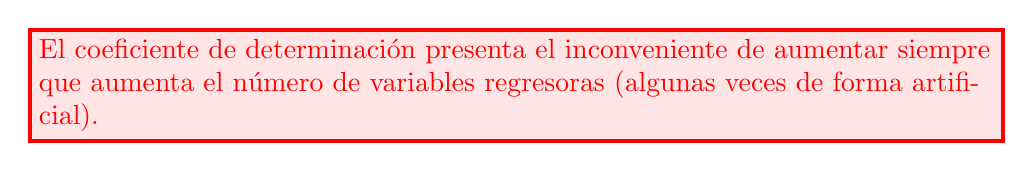
\begin{tikzpicture}
	\node[red, draw=red, fill=red!10, line width=1.5, text width=\linewidth] {El coeficiente de determinación presenta el inconveniente de aumentar siempre que aumenta el número de variables regresoras (algunas veces de forma artificial).};
\end{tikzpicture}
\subsubsection{Coeficiente de determinación ajustado}
Para penalizar el número de variables regresoras que se incluyen en el modelo de regresión, es conveniente utilizar el coeficiente de determinación corregido por el número de grados de libertad, denominado \lb{coeficiente de determinación ajustado}, definido como: \[ \overline{R}^2=1-\dfrac{\frac{SCR}{n-k-1}}{\frac{SCT}{n-1}} \]
O equivalente, \[ \overline{R}^2=1-(1-R^2)\dfrac{n-1}{n-k-1} \]
\subsection{Extensiones del modelo de regresión múltiple}
\subsubsection{Planteamiento}
El modelo de regresión lineal se puede usar para añadir variables a nuestro modelo inicial (univariante o multivariante).

El modelo más típico es el modelo polinómico: \[ h_\theta(x)=\theta_0+\theta_1x+\cdots+\theta_gx^g, \] donde el entero $g$ representa el grado del polinomio que consideremos más adecuado.

\begin{itemize}
	\item En el modelo de regresión lineal multivariante consideraremos: \[ X_1=X,X_2=X^2,\dots,X_g=X^g \]
\end{itemize}
\lb{Otro ejemplo:} Si queremos predecir $Y$ a partir de $X_1,X_2$ y $X_3$, pero el modelo lineal no funciona bien, podemos considerar el modelo: \[ h_\theta(x)=\theta_0+\theta_1x_1+\theta_2x_2+\theta_3x_3+\theta_4x_1x_2+\theta_5x_1x_3+\theta_6x_2x_3. \]
Las gráficas bidimensionales (nubes de puntos) nos pueden dar una idea de las relaciones que pueden mejorar nuestras estimaciones.
\subsubsection{Problema de sobreajuste (\texttt{\textbf{overfitting}})}
Es evidente que aumentando el grado de la regresión polinómica, disminuirá el valor de $J$.

Si no hay más de un dato para cada $x$ y consideramos $g=n$ podemos conseguir un ajuste prefecto (interpolación polinómica).
\begin{itemize}
	\item Sin embargo, este ajuste perfecto para los datos de la muestra de entrenamiento, no tiene por qué funcionar mejor cuando lo usemos en otros datos.
	\item De hecho, casi siempre funciona peor.
\end{itemize}
También se nos puede dar el caso contrario, denominado subajuste (\code{underfitting})
\subsubsection*{Un caso sencillo}
Para ilustrar este hecho consideremos un caso sencillo en el que ajustamos a los datos una recta (\code{underfitting}), un polinomio cúbico y un polinomio de orden $g=n$ (\code{overfitting}).

\begin{lstlisting}
par(mfrow = c(1,3))
x = seq(-1, 1, 0.25)
y = c(1.93, 0.73, -0.40, -0.46, 1.24, 1.78, 3.80, 3.31, 1.09)

model1 = lm(y ~ x)
r2.model1 = summary(model1)$r.squared
model2 = lm(y ~ x + I(x^2) + I(x^3))
r2.model2 = summary(model2)$r.squared
model3 = lm(y ~ x + I(x^2) + I(x^3) +  I(x^4) + I(x^5) +  I(x^6) + I(x^7) + I(x^8))
r2.model3 = summary(model3)$r.squared

x1 = seq(-1, 1, length = 50)

plot(x, y, type = "p", col = "blue", cex = 3, pch = 15, main = "Recta", cex.lab = 3, cex.axis = 3, cex.main = 3)
lines(x1, predict(model1, newdata = data.frame(x = x1)), col = "red", lwd = 4, lty = 1, cex = 0.2)
text(-0.75, 3.5, bquote(R^2 == .(format(r2.model1, digits = 3))), adj = c(0, 0), cex = 3)
plot(x, y, type = "p", col = "blue", cex = 3, pch = 15, main = "Polinomio de grado 3", cex.lab = 3, cex.axis = 3, cex.main = 3)
lines(x1, predict(model2, newdata = data.frame(x = x1)), col="purple", lwd=4, lty = 1, cex = 0.2)
text(-0.75, 3.5, bquote(R^2 == .(format(r2.model2, digits = 3))), adj = c(0, 0), cex = 3)
plot(x, y, type = "p", col ="blue", cex = 3, pch = 15, main = "Polinomio de orden 8", cex.lab = 3, cex.axis = 3, cex.main = 3)
lines(x1, predict(model3, newdata = data.frame(x = x1)), col = "green4", lwd = 4, lty = 1, cex = 0.2)
text(-0.75, 3.5, bquote(R^2 == .(format(r2.model3, digits = 3))), adj = c(0, 0), cex = 3)
\end{lstlisting}

\begin{center}
	\includegraphics[width=\linewidth]{"Temas/Imágenes/Tema 2/000020"}
\end{center}
\subsubsection*{Otro ejemplo}
Ajustamos a unos datos una recta, una parábola y un polinomio cúbico.

¿Realmente se mejora el ajuste?

\begin{lstlisting}
par(mfrow = c(1,3))
x = 1:7
y = c(3.2, 4.1, 7.5, 9.9, 10.5, 12.2, 17)

model1 = lm(y ~ x)
r2.model1 = summary(model1)$r.squared
model2 = lm(y ~ x + I(x^2))
r2.model2 = summary(model2)$r.squared
model3 = lm(y ~ x + I(x^2) + I(x^3))
r2.model3 = summary(model3)$r.squared

x1 = seq(1, 7, length = 50)

plot(x, y, type = "p", col = "blue", cex = 3, pch = 15, main = "Recta", cex.lab = 3, cex.axis = 3, cex.main = 3)
lines(x1, predict(model1, newdata = data.frame(x = x1)), col = "red", lwd = 4, lty = 1, cex = 0.2)
text(2, 16, bquote(R^2 == .(format(r2.model1, digits = 3))), adj = c(0, 0), cex = 3)
plot(x, y, type = "p", col = "blue", cex = 3, pch = 15, main = "Parábola", cex.lab = 3, cex.axis = 3, cex.main = 3)
lines(x1, predict(model2, newdata = data.frame(x = x1)), col="purple", lwd=4, lty = 1, cex = 0.2)
text(2, 16, bquote(R^2 == .(format(r2.model2, digits = 3))), adj = c(0, 0), cex = 3)
plot(x, y, type = "p", col ="blue", cex = 3, pch=15, main = "Polinomio cúbico", cex.lab = 3, cex.axis = 3, cex.main = 3)
lines(x1, predict(model3, newdata = data.frame(x = x1)), col = "green4", lwd = 4, lty = 1, cex = 0.2)
text(2, 16, bquote(R^2 == .(format(r2.model3, digits = 3))), adj = c(0, 0), cex = 3)
\end{lstlisting}

\begin{center}
	\includegraphics[width=\linewidth]{"Temas/Imágenes/Tema 2/000030"}
\end{center}
\subsubsection*{Para nuestro ejemplo}
¿Cómo se comporta el coeficiente de determinación ajustado?

¿Qué modelo seleccionaría?

\begin{lstlisting}
par(mfrow = c(1,3))
x = 1:7
y = c(3.2, 4.1, 7.5, 9.9, 10.5, 12.2, 17)

model1 = lm(y ~ x)
r2.model1 = summary(model1)$r.squared
adj.r2.model1 = summary(model1)$adj.r.squared
model2 = lm(y ~ x + I(x^2))
r2.model2 = summary(model2)$r.squared
adj.r2.model2 = summary(model2)$adj.r.squared
model3 = lm(y ~ x + I(x^2) + I(x^3))
r2.model3 = summary(model3)$r.squared
adj.r2.model3 = summary(model3)$adj.r.squared

x1 = seq(1, 7, length = 50)

plot(x, y, type = "p", col = "blue", cex = 3, pch = 15, main = "Recta", cex.lab = 3, cex.axis = 3, cex.main = 3)
lines(x1, predict(model1, newdata = data.frame(x = x1)), col = "red", lwd = 4, lty = 1, cex = 0.2)
text(2, 16, bquote(R^2 == .(format(r2.model1, digits = 3))), adj = c(0, 0), cex = 3)
text(2, 14, bquote(Adj-R^2 == .(format(adj.r2.model1, digits = 3))), adj = c(0, 0), cex = 3)
plot(x, y, type = "p", col = "blue", cex = 3, pch = 15, main = "Parábola", cex.lab = 3, cex.axis = 3, cex.main = 3)
lines(x1, predict(model2, newdata = data.frame(x = x1)), col="purple", lwd=4, lty = 1, cex = 0.2)
text(2, 16, bquote(R^2 == .(format(r2.model2, digits = 3))), adj = c(0, 0), cex = 3)
text(2, 14, bquote(Adj-R^2 == .(format(adj.r2.model2, digits = 3))), adj = c(0, 0), cex = 3)
plot(x, y, type = "p", col ="blue", cex = 3, pch = 15, main = "Polinomio cúbico", cex.lab = 3, cex.axis = 3, cex.main = 3)
lines(x1, predict(model3, newdata = data.frame(x = x1)), col = "green4", lwd = 4, lty = 1, cex = 0.2)
text(2, 16, bquote(R^2 == .(format(r2.model3, digits = 3))), adj = c(0, 0), cex = 3)
text(2, 14, bquote(Adj-R^2 == .(format(adj.r2.model3, digits = 3))), adj = c(0, 0), cex = 3)
\end{lstlisting}

\begin{center}
	\includegraphics[width=\linewidth]{"Temas/Imágenes/Tema 2/000040"}
\end{center}
\subsection*{¿Cómo evitar estos problemas?}
\subsubsection*{Procedimiento para muestras grandes}
¿Cómo elegir el número óptimo de variables? ¿Y cúales son las más adecuadas?
\begin{itemize}
	\item Separaremos nuestra muestra (de forma aleatoria) en dos grupos.
	\begin{itemize}
		\item El primer grupo se usará para estimar los coeficientes óptimos para cada $g$.
		\item El segundo grupo se utilizará para calcular los errores cuadráticos medios para cada $g$.
		\begin{itemize}[label=$\to$]
			\item Obviamente, escogeremos el grado (o grupo de variables) con menor error.
			\item De nuevo ese error nos dará una estimación menor del error real que se obtendrá con ese $g$ óptimo.
		\end{itemize}
	\end{itemize}
	\item Para hacernos una idea del error real deberemos guardar un tercer grupo de datos para calcular el error en ellos.
\end{itemize}
El número de datos en cada grupo dependen de muchos factores:
\begin{itemize}
	\item Tamaño muestral $n$.
	\item Número de variables consideradas $k$.
	\item Tiempo de programación, etc.
\end{itemize}
Por ejemplo, si tenemos $n=100$ datos, podríamos dividir el conjunto en:
\begin{itemize}
	\item Un subconjunto con 60 datos para el cálculo de $h$.
	\item Un subconjunto con 20 datos para determinar el $g$ óptimo.
	\item Un subconjunto con los otros 20 para estimar el error real en las predicciones futuras.
\end{itemize}
Si nuestra muestra tienen pocos datos, para aplicar este procedimiento deberemos aplicarlo a cada dato eliminándolo del procedimiento para estimar $h$.